\documentclass[11pt]{article}
\usepackage{natsci}
%*******************************************************************************
% polyglossia settings
%*******************************************************************************
\setdefaultlanguage[variant=british]{english}
\setotherlanguage{czech}
%*******************************************************************************
% fontspec settings
%*******************************************************************************
\setmainfont{Latin Modern Roman}[SmallCapsFont={Latin Modern Roman Caps}]
\setsansfont{Latin Modern Sans}
\setmonofont{Latin Modern Mono}
\newfontfamily{\cjkfont}{Noto Serif CJK SC}
\newfontfamily{\libertinussans}{Libertinus Sans}
%*******************************************************************************
% ucharclasses settings
%*******************************************************************************
\setTransitionsForCJK{\begingroup\cjkfont}{\endgroup}
%*******************************************************************************
% unicode-math settings
%*******************************************************************************
\setmathfont{Latin Modern Math}
\setmathfont{STIX Two Math}[range={"29B5}] % Taking the "standard symbol" (\circlehbar) from STIX Two Math
%*******************************************************************************
% geometry settings
%*******************************************************************************
\geometry{a4paper}
\geometry{margin=2cm}
\geometry{top=3cm}
\geometry{bottom=3cm}
%*******************************************************************************
% graphicx settings
%*******************************************************************************
\graphicspath{ {figures/} }
%*******************************************************************************
% fancyhdr settings
%*******************************************************************************
\pagestyle{fancy} % Make pages fancy
\fancyhf{}
\fancyhead[L]{\texttt{natsci} --- Gallery}
\fancyfoot[C]{\thepage}
%*******************************************************************************
% Changing footnotes to symbols to avoid confusion with superscript references
%*******************************************************************************
\renewcommand{\thefootnote}{\fnsymbol{footnote}}
%*******************************************************************************
% Setting paragraph indents and skips
%*******************************************************************************
\setlength{\parindent}{0pt}
\setlength{\parskip}{0.5em}
%*******************************************************************************
% siunitx settings
%*******************************************************************************
\sisetup{
    output-decimal-marker = {.},
    exponent-product = \ensuremath{{}\times{}},
    inter-unit-product = {\,}
}
%*******************************************************************************
% biblatex settings
%*******************************************************************************
\usepackage[backend=biber,style=chem-rsc,doi=true,isbn=true]{biblatex}
\addbibresource{library.bib}
%*******************************************************************************
% Title page
%*******************************************************************************
\title{\texttt{natsci} --- Gallery}
\author{Adam Přáda}
\date{2020-10-26}
%*******************************************************************************
% Other packages
%*******************************************************************************
\usepackage{hologo} % For LaTeX and other logos
\begin{document}
\pagestyle{fancy}
\maketitle



\section{Text}
Normal text is written as it is
and line breaks
in
the
code
are treated only as spaces. The number of spaces                            between words does not matter.

However, a completely empty line signifies a new paragraph. Note that it must be completely empty (may contain only spaces). Any comments or commands count as non-empty. \par Alternatively, a new paragraph can be created by a command, but that is usually not necessary. Sometimes\\ you want a line break without a new paragraph. That is done using two backslashes.

\subsection{Text styles}
Different styles of text are \textbf{bold}, \textit{italics}, \emph{emphasised} (usually italics, but can be globally changed and can react to its surroundings, e.g.\ \textit{change to \emph{upright} if the surrounding text is in italics}), \textbf{\textit{bold italics}}.

\subsection{Fonts}
Fonts can be changed using the commands crated using the \texttt{newfontfamily} command as done in the header. {\libertinussans For example this text is in Libertinus Sans.} Note the curly braces, which limit the scope of the command.

\subsection{Unicode characters}
The package uses \hologo{XeLaTeX}, which can directly typeset the whole of Unicode. However, the characters need to be supported by the font, and there is not a single font that would cover the whole of Unicode. This means that one would have to manually switch fonts if characters outside of the body font are needed. This can be done automatically for predefined Unicode ranges using the \texttt{ucharclasses} package, as demonstrated for the Han characters (漢字) in the header of this file.

\subsection{Unicode abbreviations}
The package uses \hologo{XeLaTeX}, which can directly typeset the whole of Unicode. However, there are some characters that have shorthands consisting of \textsc{ascii} characters. These are more explicit and easier to type than the actual Unicode characters, which is why we shall use them.

\paragraph{Space sizes.} There are different sizes of spaces in typesetting which are represented by different characters in Unicode. \hologo{LaTeX} automatically inserts a larger space following a full stop. This is appropriate following a sentence, but not for other uses of full stop, e.g.\ in abbreviations. There, the space should be escaped using a backslash, which achieves a normal sized space.
\\
\textenglish{Compare e.g. spacing to e.g.\ spacing.} This is only in English language.

\paragraph{Non-breaking spaces.} In some cases, spaces should not change into line breaks. This is done using the tilde symbol. Let's say that we don't want the initials to separate, like in A.~Přáda. This also suppresses the large spacing after a full stop that is present in English.

Dashes and hyphens are typed by 1 to 3 \textsc{ascii} hyphens. For hy-phe-na-ted words use a single one. For ranges of numbers, use two, which give you an en-dash (e.g.\ 1--2). For pauses --- em-dashes are used, which are represented by three hyphens.

\textczech{English quotation marks are created using backticks for the front and apostrophes for the back, like `this' or ``this''. Make sure that you don't use the the typewriter double quote \texttt{"}, which can cause troubles. Czech quotation marks, however, are typed using the double-quote character followed by quotations as previously, like "`this"'. (This works only in Czech texts.)}

\paragraph{Non-breaking hyphens} Sometimes there are hyphenated words that should not be split across lines. We use the \texttt{extdash} package and the hyphens are done as follows: 2\=/propanol.\label{importantsection}

\subsection{Text size}
There are some predefined commands for changing the text size, but you can choose an arbitrary value. Note the curly braces limiting the scope of the command.

{\Huge Huge}
{\huge huge}
{\LARGE LARGE}
{\Large Large}
{\large large}
{\normalsize normalsize}
{\small small}
{\footnotesize footnotesize}
{\scriptsize scriptsize}
{\tiny tiny}

{\fontsize{1.2cm}{1.7cm}\selectfont custom size\\ and leading\par}
% font size + leading, note that the change in leading happens only when a paragraph is ended, therefore, add \par before the closing curly brace if necessary.

% These commands act within given scope. In this case it is given by {}
% Can also change and change back or use only within a different object

\section{References}
You can refer to other places in the document using the \texttt{\textbackslash ref} command. This refers to a place labelled with the appropriate \texttt{\textbackslash label} command. This refers to section \ref{importantsection} on page \pageref{importantsection}. If these labels are inside numbered environments like sections, subsections, equations, figures or tables, they carry the appropriate number in the \texttt{ref} command and the page number in the \texttt{pageref} command. It is customary to name labels with prefixes \texttt{eq:}, \texttt{fig:} and \texttt{tab:} for equations, figures and tables respectively.

\section{Floating elements --- Figures and tables}

\begin{figure} [htp!]
    % h = here
    % t = top of page, can do 'b' for bottom
    % p = separate figure page
    % ! = override default LaTeX settings
    % LaTeX automatically chooses from the options that we list
    \centering
    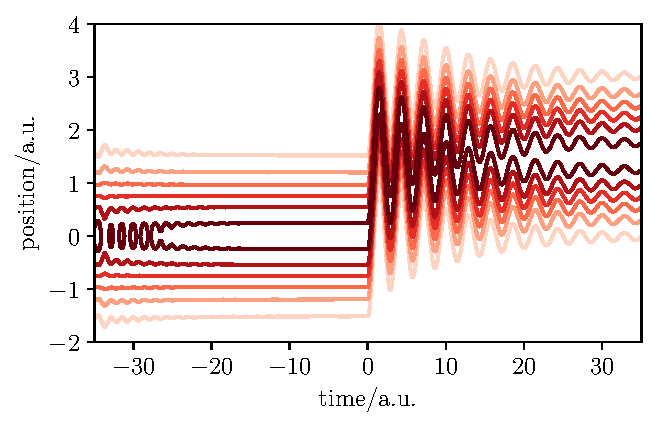
\includegraphics [width=11cm]{qheom_contour.pdf}
    \caption{
        A contour plot of a wavepacket being equilibrated with a bath in a harmonic potential centered at $q=0$. At $t=0$ the potential is shifted by an addition of a linear term, which creates a new minimum at $q=3/2$~a.u. This is a reproduction of a similar calculation from Tanimura, Wolynes, \emph{Phys.~Rev.~A}, 1991, \textbf{43}, 4131–4142.
    }
    \label{fig:qheom_contour}
\end{figure}

\section{Literature citations}
For citations, the package recommended today, is \texttt{biblatex} with \texttt{biber} backend. The citations are then imported from a separate \texttt{.bib} file, which can be automatically generated from a citation manager, like Zotero, Mendeley or EndNote.

AS citation commands, one can use either superscripts, which is mainly when the reference is not explicitly a part of the sentence.\supercite{cit1} Alternatively, you can mention them in sentence, like ref \cite{cit2}. You can also reference in full like \fullcite{mendelejev} or in a footnote like this.\footfullcite{iupac}
\printbibliography


\section{Mathematical symbols}
In math mode, numbers are upright and Latin and Greek letters are by default typeset in italics
\[
x=2\Xi
\]
Basic mathematical operations are
\[
y = 1 + x - 5^3 + 6/7 + \frac{5}{6} \times 8 + 5 \cdot 3
\]
Brackets and parentheses are typed as shown below. Note the self-adjusting left and right brackets.
\[
f(x),\ \mathrm{FT}[f],\ O = \{1,2,3\}, (\frac{5}{6}),\ \left(\frac{5}{6}\right),\ [\frac{5}{6}],\ \left[\frac{5}{6}\right],\ \{\frac{5}{6}\},\ \left\{\frac{5}{6}\right\}
\]
Note that left and right commands need to be on the same line, if you need to split the bracket across two lines, use these manual commands
\begin{multline}
    f = \Biggl[  \biggl[ \Bigl[ \bigl[ \frac{5}{6}\\
    + \frac{8}{9} \bigr] \Bigr] \biggr] \Biggr]
\end{multline}
To access the different Unicode alphabets, use the following commands:
\begin{align*}
    &a A \xi \Xi                &
    &\symnormal{a A \xi \Xi}    &
    &\symliteral{a A \xi \Xi}   &
    &\symup{a A \xi \Xi}    & 
    &\symit{a A \xi \Xi}    &
    &\symbf{a A \xi \Xi}   &
    &\symsf{a A \xi \Xi}    &
    &\symtt{a A \xi \Xi}    \\
    &\symbfsf{a A \xi \Xi}   &
    &\symbfup{a A \xi \Xi}   &
    &\symbfit{a A \xi \Xi}   &
    &\symbb{a A \xi \Xi}   &
    &\symbbit{a A \xi \Xi}   &
    &\symcal{a A \xi \Xi}   &
    &\symbfcal{a A \xi \Xi}   &
    &\symscr{a A \xi \Xi}    \\
    &\symbfscr{a A \xi \Xi}   &
    &\symfrak{a A \xi \Xi}   &
    &\symbffrak{a A \xi \Xi}   &
    &\symsfup{a A \xi \Xi}   &
    &\symbfsfup{a A \xi \Xi}    &
    &\symsfit{a A \xi \Xi}    &
    &\symbfsfit{a A \xi \Xi} \\
\end{align*}
There are also legacy \LaTeX{} font commands, which are appropriately redefined in \texttt{unicode-math}. They behave actually differently in \texttt{unicode-math}. While the \texttt{sym} commands output actually uses the Unicode mathematical alphabets and should be used for variables, the \texttt{math} commands (at least roman, italic, bold) uses the text fonts and should be used for operator names (e.g.\ one could get a ligature between letters in an operator name, but not between variables). However, for labels and words, the environment \texttt{text} should be used, like in
\[
H_\text{fus}^\std,\ m_\text{glucose}
\]

\begin{table}[H]
    \caption{New \texttt{unicode-math} commands which overlap with legacy
        math commands. For new documents the \texttt{sym} versions are recommended.}
    \centering
    \begin{tabular}[t]{ll}
        \toprule
        Command & Synonym \\
        \midrule
        \texttt{symnormal}  & \texttt{mathnormal} \\
        \texttt{symliteral} &                 \\
        &  \\
        &  \\
        &  \\
        \texttt{symbb}      & \texttt{mathbb}     \\
        \texttt{symbbit}    & \texttt{mathbbit}   \\
        \texttt{symcal}     & \texttt{mathcal}    \\
        \texttt{symscr}     & \texttt{mathscr}    \\
        \texttt{symfrak}    & \texttt{mathfrak}   \\
        \texttt{symsfup}    & \texttt{mathsfup}   \\
        \texttt{symsfit}    & \texttt{mathsfit}   \\
        \bottomrule
    \end{tabular}\qquad
    \begin{tabular}[t]{ll}
        \toprule
        Command & Synonym \\
        \midrule
        &  \\
        &  \\
        \texttt{symbfsf}    & \texttt{mathbfsf}   \\
        \texttt{symbfup}    & \texttt{mathbfup}   \\
        \texttt{symbfit}    & \texttt{mathbfit}   \\
        &  \\
        &  \\
        \texttt{symbfcal}   & \texttt{mathbfcal}  \\
        \texttt{symbfscr}   & \texttt{mathbfscr}  \\
        \texttt{symbffrak}  & \texttt{mathbffrak} \\
        \texttt{symbfsfup}  & \texttt{mathbfsfup} \\
        \texttt{symbfsfit}  & \texttt{mathbfsfit} \\
        \bottomrule
    \end{tabular}
\end{table}

For many operators, macros are predefined, which makes correct typesetting easy. New operators can be defined using \texttt{DeclareMathOperator} from the \texttt{amsmath} package.
\[
\sin(x),\ \cosh(x),\ \exp(x),\ \log(x),\ \sqrt{x},\ \sqrt[3]{x},\ \sum_{n=0}^{N} Q_n,\ \int_{0}^{1} f(x) \ud x,\ \prod_{n=0}^{N} Q_n
\]

\section{Mathematical equations}
\hologo{LaTeX} has a special math mode that needs to be triggered by a command.

Inline mathematics is written either using dollar signs like this $x=y$ (this is the old \TeX{} macro) or using escaped parentheses \(x=y\). These two are completely equivalent, even though the latter one is somewhat neater and makes it easier to search for a missing one.

Display mathematics is written either using escaped brackets.
\[
x=y
\]
or using the \texttt{equation*} environment.
\begin{equation*}
    x=y
\end{equation*}
These two are equivalent. The * means that the equation is not automatically numbered. Please refrain from using the old \TeX{} double dolar macro \texttt{\$\$ x=y \$\$}. This is poorly defined and breaks things. For automatically numbered equations, use the \texttt{\textbackslash equation} environment.
\begin{equation}
    x=y
\end{equation}

Note that empty lines prior to \texttt{\textbackslash[} or \texttt{\textbackslash begin\{equation\}} matter. Display equations are parts of paragraphs or paragraphs themselves, and the spacing reflects this. Also, note that spaces can be used to separate individual commands, but just like in normal mode, any number of spaces counts as a single space. 

If you want to number equations manually, you use the \texttt{tag} command
\[
x=y
\tag{4}
\]

Other environments that you may want to use are \texttt{align} (aligned equations, arrays of equations), \texttt{multline} (not a typo) (one equation split across line) and \texttt{gather} (not-aligned equations, one per line). (Please don't use \texttt{array}, it causes problems.)

To split one long equation across lines, use the \texttt{multline} environment.
\begin{multline}
    \diffp{b(Q_0,P_0,t)}{t} = \left[\frac{P_0}{m}\diffp{}{Q_0} - \frac{\ud F(Q_0)}{\ud Q_0}\diffp{}{P_0}\right] b(Q_0,P_0,t) \\
    + \alpha_M \int \ud \vc{Q'}\int\ud \vc{P'}\ \ue^{-\beta H_M(\vc{Q},\vc{P})}\ue^{\ui\beta \theta(\vc{Q},\vc{P})} F_{\mathrm{fluct}}(\vc{Q})\diffp{}{P_0}\ue^{\mathcal{L}_M t}B_N(\vc{Q}),
\end{multline}

To have an equation with different cases
\begin{equation}
    T_{ln}=
    \begin{cases}
        1, & n=0, \\
        \sqrt{2}\sin(2\pi ln/N), & n = 1, \cdots, (N-1)/2, \\
        \sqrt{2}\cos(2\pi ln/N), & n = -1, \cdots, -(N-1)/2.
    \end{cases}
\end{equation}

If you want to have multiple equations in the same environment, each individually numbered, use \texttt{gather}
\begin{gather}
    -\frac{\ui}{\hbar} \hat{H}^\times \hat{\rho} \longrightarrow
    -\hat{\mathcal{L}}_\mathrm{W} W(q,p),\\
    \hat{\rho} \longrightarrow W(q,p) +\diffp{}{p} W(q,p),\\
    -\frac{\mathrm{i}}{\hbar} \hat{q}^\times \hat{\rho} \longrightarrow +\diffp{}{p} W(q,p),\\
    \hat{q}^\circ \hat{\rho} \longrightarrow 2qW(q,p),
\end{gather}
If you think that they would look better aligned, use \texttt{align}
\begin{align}
    -\frac{\mathrm{i}}{\hbar} \hat{H}^\times \hat{\rho} &\longrightarrow
    -\hat{\mathcal{L}}_\mathrm{W} W(q,p),\\
    \hat{\rho} &\longrightarrow W(q,p) +\diffp{}{p} W(q,p),\\
    -\frac{\mathrm{i}}{\hbar} \hat{q}^\times \hat{\rho} &\longrightarrow +\diffp{}{p} W(q,p),\\
    \hat{q}^\circ \hat{\rho} &\longrightarrow 2qW(q,p),
\end{align}
Align can also be used for arrays of equations or expressions like

\begin{align*}
    &\num{12345,67890}                                 &
    &\num[output-decimal-marker = {,}]{12345,67890}    &
    &\num{1+-2i}                                       \\
    &\num{0.3e45}                                      &
    &\num[exponent-product = \ensuremath{{}\cdot{}}]{0.3e45}            &
    &\si{kJ.mol^{-1}}                                  \\
    &\SI{15.3}{\joule\per\mole\per\kelvin}             &
    &\SI[inter-unit-product = \ensuremath{{}\cdot{}}]{15.3}{\J\mol\K} &
    &\SI{1525.3}{kJ.mol^{-1}}                          \\
    &\ang{4,5}                                         &
    &\ang{1;2;3}                                       &
\end{align*}
If you want to have aligned multiple equations under one equation number, use \texttt{split}
\begin{equation}
    \begin{split}
        C_0 &= \frac{\hbar\eta\gamma^2}{2}\left[\cot\left(\frac{\beta\hbar\gamma}{2}\right) -\mathrm{i}\right],\\
        C_{k>0} &= \frac{2\eta\gamma^2}{\beta}\frac{\gamma_k}{\gamma_k^2-\gamma^2}.
    \end{split}
\end{equation}


\subsection{Footnotes}
Footnotes are simple done like this.\footnote{My first footnote.} You can write the footnote text\footnotemark outside of the paragraph, if appropriate.
\footnotetext{My second footnote}



\section{Mathematical typesetting conventions}
The document uses \texttt{unicode-math}, which means that you can type mathematical symbols directly using their Unicode characters. However, since there are no Unicode keyboards, it is usually more convenient to use the related \textsc{ascii} macros.

\paragraph{Variables} All variables are typeset in \textit{italics/slanted/oblique}. This includes fundamental constants that do not vary. (We can imagine a hypothetical situation when they do.)
\[
x, y, i, j, e\ (\text{elementary charge}), c\ (\text{the speed of light})
\]
Vector variables are typeset in \textbf{\textit{bold italics}}. (They are still variables.) For this, use the \texttt{vc} command.
\[
\vc{F} = m \vc{a}
\]
Matrix/tensor variables are typeset in bold sans-serif font. For these the command \texttt{mat} was defined. (In addition, a command \texttt{transp} was defined for transpose \transp)
\[
\vc{c}^\transp \mat{H} \vc{c} = E
\]
\paragraph{Non-variables} All other objects, like operators, labels, abbreviations, function names or units, must be typed upright. This also applies to mathematical constants that are usually denoted by letters, like e (Euler's number), i (imaginary unit), \upi (circumference of a circle of a unit diameter). Basic functions, like trigs and logs have their own commands. For labels or phrases, \texttt{text} command is used. For differentials d, e, i and \upi, new commands were defined for their upright versions \texttt{ue, ud, ui, upi}. Similarly, the difference, the upright capital delta is used \uDelta, which has been assigned the macro \texttt{uDelta}. For derivatives, the package \texttt{diffcoeff} provides a simpler notation than explicitly writing fractions. See examples below.
\[
\sin x, \ln \uDelta H_\text{fus}^\std,\int \ud x, \ue^{\ui \upi}, \mat{A}^\transp, \diff{f(x)}{x}, \diff[3]{f}{x}[x=0], \diffp[3]{f(x,y)}{x}[y]
\]
Also note the standard state symbol $\circlehbar$, which has been assigned the \texttt{std} macro.

\paragraph{Mathmatical alphabets} If you want a more direct control, below is the list of all the mathematical alphabets that exist in Unicode. (These commands can also be used without the curly braces, in which case they apply to the next symbol, like this $\symcal L$. However, with curly braces it is more explicit what you mean.)
\begin{align*}
    &a A \xi \Xi                &
    &\symnormal{a A \xi \Xi}    &
    &\symliteral{a A \xi \Xi}   &
    &\symup{a A \xi \Xi}    &
    &\symit{a A \xi \Xi}    &
    &\symbf{a A \xi \Xi}   &
    &\symsf{a A \xi \Xi}    &
    &\symtt{a A \xi \Xi}    \\
    &\symbfsf{a A \xi \Xi}   &
    &\symbfup{a A \xi \Xi}   &
    &\symbfit{a A \xi \Xi}   &
    &\symbb{a A \xi \Xi}   &
    &\symbbit{a A \xi \Xi}   &
    &\symcal{a A \xi \Xi}   &
    &\symbfcal{a A \xi \Xi}   &
    &\symscr{a A \xi \Xi}    \\
    &\symbfscr{a A \xi \Xi}   &
    &\symfrak{a A \xi \Xi}   &
    &\symbffrak{a A \xi \Xi}   &
    &\symsfup{a A \xi \Xi}   &
    &\symbfsfup{a A \xi \Xi}    &
    &\symsfit{a A \xi \Xi}    &
    &\symbfsfit{a A \xi \Xi} \\
\end{align*}

\paragraph{Units and decimal numbers}For the formating of numerical values and units, the package \texttt{siunitx} is used. The main advantage is the ability to globally change the decimal separator between dot and comma, or the way units are typeset. This can be used e,g,\ in making of different language versions. Therefore, all decimal numbers and numbers with units should be typeset as follows:
\begin{align*}
&\num{12345,67890}                                 &
&\num[output-decimal-marker = {,}]{12345,67890}    &
&\num{1+-2i}                                       \\
&\num{0.3e45}                                      &
&\num[exponent-product = \ensuremath{{}\cdot{}}]{0.3e45}            &
&\si{kJ.mol^{-1}}                                  \\
&\SI{1525.3}{kJ.mol^{-1}}                          &
&\SI{10}{\micro\metre}                             &
&\SI{10}{\um}                                      \\
&\SI{10}{\ul}                                      &
&\SI{10}{\degreeCelsius}                           &
&\SI{1525.3}{\kJ\per\mol}                          \\
&\SI{15.3}{\joule\per\mole\per\kelvin}             &
&\SI[inter-unit-product = \ensuremath{{}\cdot{}}]{15.3}{\J\mol\K} &
&\SI{1525.3}{kJ.mol^{-1}}                          \\
&\ang{4,5}                                         &
&\ang{1;2;3}                                       &
\end{align*}
Note that the units are correctly typeset in upright font with a non-breaking space between the number and the unit. It does not matter whether decimal comma or dot is used in the source code, the output will follow the package setting. Units can be either selected by typing their abbreviations separated by dots with explicit powers, or by specific commands as demonstrate above.

\section{Chemistry typesetting}
The package used is \texttt{chemmacros}. Chemical formulas are then enclosed in the \texttt{ch} command, like this \ch{H2O}. This works also in the math mode like in
\[
\uDelta G_\text{fus}^\std(\ch{H2O}).
\]
Alternatively, for full reactions, one can use the \texttt{reaction} and \texttt{reaction*} environments. (* again to avoid numbering)
\begin{reaction*}
    H2SO4 + 2 H2O <=> HSO4- + H3O+ + H2O <=> 2 H3O+ + SO4^{2-}
\end{reaction*}
\begin{reaction*}
    _{0}^{1}n + \isotope{235,U} -> 3 _{0}^{1}n + \isotope{93,Kr} + \isotope{140,Ba}
\end{reaction*}
\begin{reaction*}
    2 R-CHO -> R-COO^{-} + R-CH2-OH
\end{reaction*}
\begin{reaction*}
    F2 + H2O \sld -> [ $\SI{-40}{\degreeCelsius}$ ] HF ($\mathbf{A}$) + HOF ($\mathbf{B}$)
\end{reaction*}
However, the package can do much more, so feel free to explore
\begin{center}
    \begin{tabular}{cc} % I am not sure if this is the easiest way of doing this
        {\large
            \ch{Ag^\fscrp} \ch{^\fscrm}\chlewis{90:180:270:}{O}\bond{sb}\ch{C}\bond{tp}\chlewis{0:}{N}
        }
        &
        {\large
            \ch{Ag^\fscrp} \ch{^\fscrm}\chlewis{90:180:270:}{O}\bond{sb}\ch{N^\fscrp}\bond{tp}\chlewis{0:}{C}\ch{^\fscrm}
        }\\
    \end{tabular}
\end{center}

\newpage
\begin{landscape}
    \subsection{A landscape page}
    \begin{figure} [htp!] %pro lepsi obplouvani textu
        \centering
        \begin{subfigure}[b]{10cm}
            \centering
            %\vspace*{-1cm}
            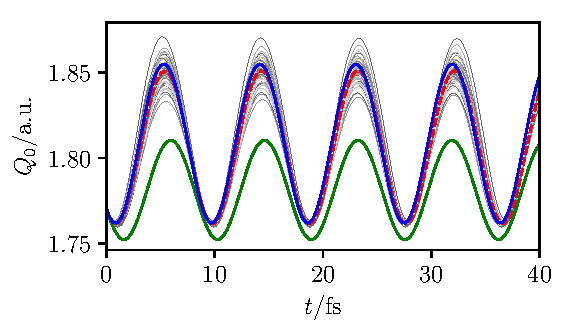
\includegraphics [scale=1]{norm.pdf}
            %\vspace*{-0.3cm}
            \caption{Typical trajectory}
        \end{subfigure}
        \begin{subfigure}[b]{10cm}
            \centering
            %\vspace*{-1cm}
            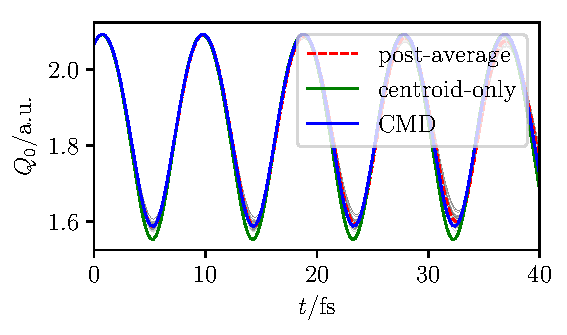
\includegraphics [scale=1]{good.pdf}
            %\vspace*{-0.3cm}
            \caption{Good agreement}
        \end{subfigure}
        \begin{subfigure}[b]{10cm}
            \centering
            %\vspace*{-0.15cm}
            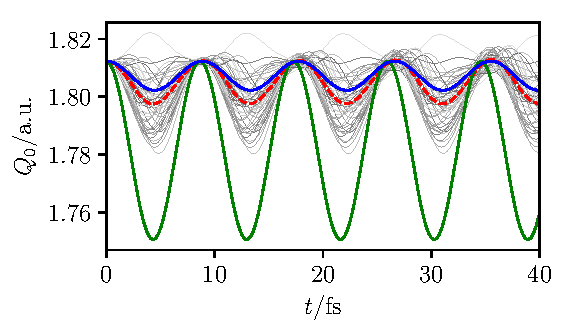
\includegraphics [scale=1]{bad.pdf}
            %\vspace*{-0.3cm}
            \caption{Poor agreement}
        \end{subfigure}
        \begin{subfigure}[b]{10cm}
            \centering
            %\vspace*{-0.1cm}
            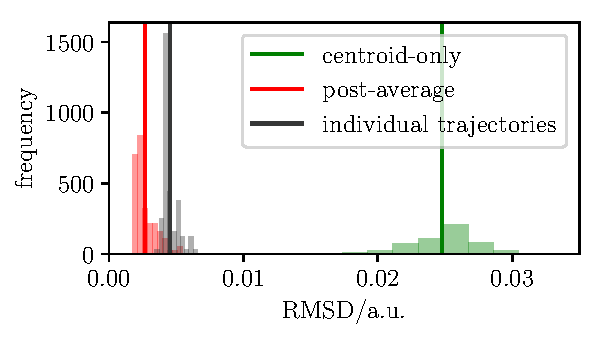
\includegraphics [scale=1]{rmsd.pdf}
            %\vspace*{-0.3cm}
            \caption{RMSD from CMD histogram at 150 K}
        \end{subfigure}
        \caption{
            From time to time it is useful to have a page or two in landscape for wide figures.
        }
    \end{figure}
\end{landscape}
\newpage
\end{document}
